\documentclass[12pt]{article}
\usepackage[margin=1in]{geometry}
\usepackage{amsmath, amssymb, amsthm, graphicx, hyperref}
\usepackage{amsmath}
\usepackage{enumerate}
\usepackage{fancyhdr}
\usepackage{multirow, multicol}
\usepackage{tikz}
\usepackage{wrapfig}
\pagestyle{fancy}
\usepackage{titlesec}
\usepackage{lastpage}
\usepackage{multirow}
\usepackage{indentfirst}
\fancyhead[LO]{JACK Z}
\fancyhead[RO]{Page \thepage\ of \pageref{LastPage}}
\usepackage{comment}
\newtheorem{definition}{Definition}
\usepackage{amsmath}
\usepackage{booktabs}
\usepackage{xcolor}
\usepackage{tcolorbox}  % For creating styled boxes
\tcbuselibrary{most}
\usepackage{tcolorbox} % for creating colored or framed text boxes
\tcbuselibrary{breakable} % allows tcolorboxes to break across pages

\definecolor{examplebg}{RGB}{255, 228, 225} % Light red background
\tcbuselibrary{theorems} 
\usepackage{graphicx}
\usepackage{booktabs} % For better table formatting
\usepackage{caption} % Essential for \captionof
\usepackage{tcolorbox} % For creating colored boxes
\tcbuselibrary{most} % Load most libraries for tcolorbox

\newtcbtheorem[number within=subsection]{Note}{Note}{
    colback=Black!5,
    colframe=white!35!black,
    fonttitle=\bfseries,
    colbacktitle=blue!85!black,
    coltitle=white,
    enhanced,
    attach boxed title to top left={yshift=-2mm, xshift=2mm},
    boxed title style={sharp corners},
    sharp corners
}{Not}

\newtcbtheorem[number within=subsection]{Definition}{Definition}{
    colback=blue!5,
    colframe=blue!35!black,
    fonttitle=\bfseries,
    colbacktitle=blue!85!black,
    coltitle=white,
    enhanced,
    attach boxed title to top left={yshift=-2mm, xshift=2mm},
    boxed title style={sharp corners},
    sharp corners
}{def}

\newtcbtheorem[number within=subsection]{mytheorem}{Theorem}{
    colback=orange!5,      % Background color of the box
    colframe=orange,     % Border color of the box
    coltitle=white,     % Color of theorem title
    colbacktitle=orange!85!black,, % Background color for the title
    fonttitle=\bfseries,
    title after break={Theorem \csname the\tcbcounter\endcsname\ -- Continued}, % for continued theorems
    enhanced,
    attach boxed title to top left={yshift=-2mm, xshift=2mm},
    boxed title style={sharp corners, colframe=black},
    sharp corners,
    separator sign none % no sign between title and theorem text
}{thm}


\usepackage{lipsum} % 生成示例文本
\usepackage{fancyhdr}

\pagestyle{fancy}
\renewcommand{\headrulewidth}{0pt} % 去掉页眉下方的横线
\fancyfoot[C]{\textcopyright\ \fcolorbox{purple}{white}{Novel Prep}}

% Define custom colors
\definecolor{deepblue}{rgb}{0.0, 0.18, 0.39}
\definecolor{deepred}{rgb}{0.6, 0, 0}

% Define theorem style
\newtheoremstyle{beautifulthm}
  {10pt} % Space above
  {10pt} % Space below
  {\itshape} % Body font
  {} % Indent amount
  {\bfseries\color{deepblue}} % Theorem head font
  {.} % Punctuation after theorem head
  {.5em} % Space after theorem head
  {} % Theorem head spec

\theoremstyle{beautifulthm}
\newtheorem{theorem}{Theorem}[section]

\begin{document}

\title{AP Calculus AB\&BC}
\author{Hongjun Zeng}
\maketitle

\lipsum[1-10] 

\newpage
\tableofcontents

\newpage

\section{Limits and Continuity}
\section{Differentiation: Definition and Fundamental Properties}
\section{Differentiation: Composite, Implicit, and Inverse Function}
\section{Application of Differentiation}
\newpage
\subsection{Interpreting the Meaning of the Derivative}
The first interpretation of a derivative is rate of change. If \( f(x) \) represents a quantity at any \( x \), then the derivative \( f'(a) \) represents the instantaneous rate of change of \( f(x) \) at \( x = a \).

\subsubsection{Units of the Derivative}
\begin{mytheorem}{Units of the Derivative}{}
If \( y \) is a function of \( x \), that is,
\( y = f(x) \) for some function \( f \), and \( y \) is measured in feet and \( x \) in seconds, then the units of
\( y' = f' \) are "feet per second," commonly written as "ft/s." In general, if \( y \) is measured in units \( P \) and \( x \) is measured in units \( Q \), then \( y' \) will be measured in units "P per Q," or "P/Q."

Here we see the fraction-like behavior of the derivative in the notation:
\[
\text{the units of } \frac{dy}{dx} \text{ are } \frac{\text{units of } y}{\text{units of } x}.
\]
\end{mytheorem}

\begin{minipage}{\linewidth}
    \centering
    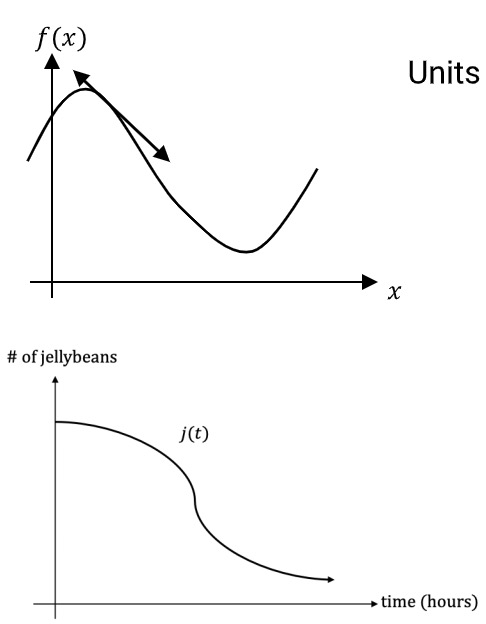
\includegraphics[width=0.28\linewidth]{Example_16.jpg} % Adjust the image width as necessary
    \captionof{figure}{}
    \label{fig:graph}
\end{minipage}

\begin{tcolorbox}[colback=examplebg, colframe=red!75!black, title=\textbf{EXAMPLE 1: The meaning of the derivative: Manufacturing}, fonttitle=\bfseries, sharp corners]
What do \( P(1000) = 500 \) and \( P'(1000) = 0.25 \) mean? Approximate \( P(1100) \).

\tcblower
\textbf{Solution:}  
The equation \( P(1000) = 500 \) means that selling 1,000 widgets returns a profit of \$500. We interpret \( P'(1000) = 0.25 \) as meaning that the profit is increasing at a rate of \$0.25 per widget (the units are "dollars per widget"). Since we have no other information to use, our best approximation for \( P(1100) \) is:
\[
P(1100) \approx P(1000) + P'(1000) \cdot 100 = 500 + 100 \cdot 0.25 = 525. \tag{2.2.2}
\]

We approximate that selling 1,100 widgets returns a profit of \$525.
\end{tcolorbox}

\newpage
\subsection{Straight Line Motion(Position, Velocity, and Acceleration)}
\begin{mytheorem}{Straight Line Motion}{}
\begin{enumerate}
    \item If \( s = f(t) \) is the position function of a particle moving in a straight line:
    \[
    \frac{\Delta s}{\Delta t} \text{ represents the average velocity over a time period } \Delta t.
    \]

    \item The instantaneous velocity, which is the rate of change of displacement with respect to time, is given by:
    \[
    v = \frac{ds}{dt} = s'(t)
    \]

    \item The instantaneous rate of change of velocity with respect to time, known as acceleration, is given by:
    \[
    a(t) = v'(t) = s''(t).
    \]
\end{enumerate}
\end{mytheorem}

\begin{minipage}{\linewidth}
    \centering
    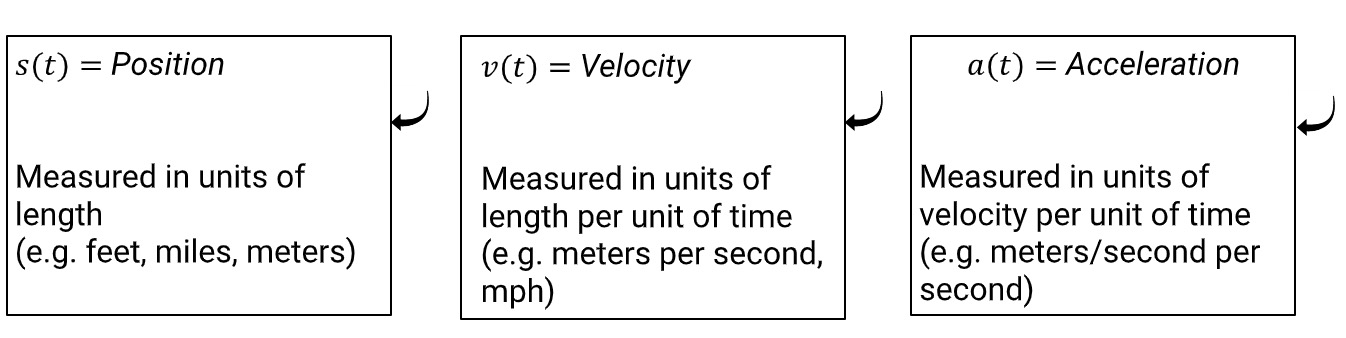
\includegraphics[width=1.0\linewidth]{Example_17.jpg} % Adjust the image width as necessary
    \captionof{figure}{}
    \label{fig:graph}
\end{minipage}
    \item \textbf{Velocity as a Vector:} 
    Velocity is a vector quantity, meaning it has both magnitude (speed) and direction. 
    
\begin{Note}{Turning Left or Right: Velocity and Direction}{}

\begin{itemize}

    \item \textbf{Turning Left:}
    When an object turns left, its velocity vector rotates \textbf{counterclockwise} in the coordinate plane. ($v(t)$ is \textbf{Negative})

        \item \textbf{Turning Right:}
    When an object turns Right, its velocity vector rotates \textbf{clockwise} in the coordinate plane. ($v(t)$ is \textbf{Positive})
\end{itemize}


\end{Note}



\begin{Note}{Speeding up/down?}{}

\begin{itemize}
    \item An object is \textbf{speeding up} when the direction of the acceleration matches the direction of the velocity (acceleration and velocity have the same sign).
    \item An object is \textbf{slowing down} when the direction of the acceleration and velocity is opposite (acceleration and velocity have opposite signs).
\end{itemize}


\end{Note}

\begin{tcolorbox}[colback=examplebg, colframe=red!75!black, title=\textbf{EXAMPLE 1:  Position of a particle}, fonttitle=\bfseries, sharp corners]
A particle moves along the \( x \)-axis. The position of the particle, in feet, is given by:
\[
x(t) = \frac{1}{3}t^3 - \frac{5}{2}t^2 + 4t + 6, \quad 0 \leq t \leq 5,
\]
where \( t \) is measured in minutes.
\begin{enumerate}
    \item[(a)] When is the particle at rest?
    \item[(b)] When is the particle moving toward the left?
    \item[(c)] At \( t = 3 \), is the particle speeding up or slowing down? Justify your answer.
\end{enumerate}
\tcblower
\textbf{Solution}
\begin{enumerate}
    \item[(a)] The particle is at rest when the velocity is zero. The velocity is the derivative of the position function:
    \[
    v(t) = \frac{dx}{dt} = t^2 - 5t + 4.
    \]
    Setting \( v(t) = 0 \):
    \[
    t^2 - 5t + 4 = 0 \implies (t - 4)(t - 1) = 0.
    \]
    Thus, the particle is at rest at \( t = 1 \, \text{minute} \) and \( t = 4 \, \text{minutes.} \)

    \item[(b)] The particle is moving toward the left when the velocity is negative (\( v(t) < 0 \)). From the factorization:
    \[
    v(t) = (t - 4)(t - 1),
    \]
    we analyze the intervals:
    \begin{itemize}
        \item \( t < 1 \): \( v(t) > 0 \) (positive velocity).
        \item \( 1 < t < 4 \): \( v(t) < 0 \) (negative velocity).
        \item \( t > 4 \): \( v(t) > 0 \) (positive velocity).
    \end{itemize}
    Thus, the particle moves toward the left during the interval \( 1 < t < 4 \, \text{minutes.} \)

    \item[(c)] At \( t = 3 \), the acceleration is the derivative of the velocity:
    \[
    a(t) = \frac{dv}{dt} = 2t - 5.
    \]
    At \( t = 3 \):
    \[
    v(3) = (3 - 4)(3 - 1) = -1 \cdot 2 = -2 \, \text{ft/min},
    \]
    \[
    a(3) = 2(3) - 5 = 6 - 5 = 1 \, \text{ft/min}^2.
    \]
    The velocity is negative and the acceleration is positive, so the particle is slowing down (the acceleration opposes the velocity).
\end{enumerate}




\end{tcolorbox}




\begin{tcolorbox}[colback=examplebg, colframe=red!75!black, title=\textbf{EXAMPLE 2:  Position of a particle}, fonttitle=\bfseries, sharp corners]
The position of a particle is given by the equation:
\[
s = f(t) = t^3 - 6t^2 + 9t,
\]
where \( t \) is measured in seconds and \( s \) in meters.
\begin{enumerate}
    \item[(a)] Find the velocity at time \( t \).
    \item[(b)] What is the velocity after \( 2 \, \text{seconds}? \) After \( 4 \, \text{seconds}? \)
    \item[(c)] When is the particle at rest?
    \item[(d)] When is the particle moving forward (that is, in the positive direction)?
    \item[(e)] Draw a diagram to represent the motion of the particle.
    \item[(f)] Find the total distance traveled by the particle during the first \( 5 \, \text{seconds.} \)
    \item[(g)] Find the acceleration at time \( t \) and after \( 4 \, \text{seconds.} \)
    \item[(h)] When is the particle speeding up, and when is it speeding down?
\end{enumerate}




\end{tcolorbox}




\newpage
\subsection{Rates of Change in Applied Contexts Other Than Motion}


\begin{Definition}{Rate of Change}{}

\begin{itemize}

    \item The rate of change function is the \textbf{derivative} of the original function.
    \begin{itemize}
        \item Derivative notation is not always used! For example, \( A(t) \) could represent the rate at which water fills a container.
        \item The rate of change function can be presented as a graph, table, or equation.
    \end{itemize}
\end{itemize}
\end{Definition}

\begin{itemize}
    \item A \textbf{rate of change function} helps us predict how a quantity will change over time. It answers questions such as:
    \begin{itemize}
        \item When is the quantity increasing or decreasing?
        \item When is the quantity at its maximum or minimum?
        \item How fast is the quantity changing?
    \end{itemize}
\end{itemize}


\begin{tcolorbox}[colback=examplebg, colframe=red!75!black, title=\textbf{EXAMPLE 1:Rates of Change}, fonttitle=\bfseries, sharp corners]
People enter an amusement park at a rate given by:
\[
E(t) = \frac{15600}{t^2 - 24t + 160},
\]
where \( E \) is in people per hour and \( t \) is in hours after midnight. 

\begin{itemize}
    \item Find \( E'(11) \).
    \item Using correct units, interpret the meaning of this value in the context of the problem.
\end{itemize}

\tcblower
\textbf{Solution}
The given function is:
\[
E(t) = \frac{15600}{t^2 - 24t + 160}.
\]

Using the quotient rule:
\[
E'(t) = \frac{-15600(2t - 24)}{(t^2 - 24t + 160)^2}.
\]

At \( t = 11 \):
\[
E'(11) = \frac{31200}{289} \approx 107.96.
\]

\textbf{Interpretation:} At \( t = 11 \) (11 AM), the rate of people entering the park is \textbf{increasing} by about \( 108 \, \text{people/hour}^2 \).

\end{tcolorbox}


\begin{Note}{"Rate In" and "Rate Out" }{}


\begin{itemize}
    \item Some quantities are determined by two rates: a \textbf{"rate in"} and a \textbf{"rate out."}
    \begin{itemize}
        \item The number of people at a soccer game is determined by the rate at which people enter the stadium and the rate at which people leave the stadium.
        \item The volume of water in a tank is determined by the rate at which water fills the tank and the rate at which water leaks or is drained from the tank.
    \end{itemize}

    \item To determine whether a quantity is \textbf{increasing} or \textbf{decreasing} at a specific time or interval, compare the \textbf{rate in} and \textbf{rate out}.
\end{itemize}
\end{Note}



\begin{tcolorbox}[colback=examplebg, colframe=red!75!black, title=\textbf{EXAMPLE 1:Rates of Chang}, fonttitle=\bfseries, sharp corners]
The penguin population on an island is modeled by the differentiable function \( P(t) \) for \( 0 \leq t \leq 40 \), where \( t \) is in years. There are 100,000 penguins on the island at \( t = 0 \). The birth rate for the penguins is modeled by:
\[
B(t) = 1000e^{0.06t} \, \text{penguins per year},
\]
and the death rate is modeled by:
\[
D(t) = 250e^{0.1t} \, \text{penguins per year}.
\]

\begin{enumerate}
    \item[(a)] Is the penguin population increasing or decreasing at \( t = 5 \) years? Give a reason for your answer.
\end{enumerate}

\tcblower
\textbf{Solution}
To determine whether the population is increasing or decreasing at \( t = 5 \), we compare the birth rate \( B(t) \) and the death rate \( D(t) \).

\textbf{Step 1: Evaluate \( B(5) \) and \( D(5) \)}
The birth rate at \( t = 5 \):
\[
B(5) = 1000e^{0.06(5)} = 1000e^{0.3}.
\]
Using a calculator:
\[
B(5) \approx 1349.86 \, \text{penguins per year}.
\]

The death rate at \( t = 5 \):
\[
D(5) = 250e^{0.1(5)} = 250e^{0.5}.
\]
Using a calculator:
\[
D(5) \approx 397.68 \, \text{penguins per year}.
\]

\textbf*{Step 2: Compare \( B(5) \) and \( D(5) \)}
At \( t = 5 \):
\[
B(5) > D(5) \quad \text{(1349.86 $>$ 397.68)}.
\]

\textbf{Conclusion}
Since \( B(5) > D(5) \), the birth rate exceeds the death rate at \( t = 5 \), so the penguin population is \textbf{increasing}.

\end{tcolorbox}
\newpage
\subsection{Related Rates}
\subsubsection{Introduction of Related Rates}
\begin{Note}{Finding Related Rates }{}
The Chain Rule can be used to find the rates of change of two or more related variables with respect to time.
\tcblower

For example, when water is drained from a conical tank, the volume \( V \), the radius \( r \), and the height \( h \) of the water level are related by:
\[
V = \frac{\pi}{3}r^2h.
\]

Differentiating implicitly with respect to \( t \):
\[
\frac{dV}{dt} = \frac{d}{dt} \left( \frac{\pi}{3}r^2h \right),
\]
\[
\frac{dV}{dt} = \frac{\pi}{3} \left( r^2 \frac{dh}{dt} + 2r h \frac{dr}{dt} \right).
\]

This equation shows that the rate of change of \( V \) depends on the rates of change of both \( h \) and \( r \).

\end{Note}

\begin{tcolorbox}[colback=examplebg, colframe=red!75!black, title=\textbf{EXAMPLE 1:Two Rates That Are Related}, fonttitle=\bfseries, sharp corners]
The variables \( x \) and \( y \) are both differentiable functions of \( t \) and are related by the equation:
\[
y = x^2 + 3.
\]
Find \( \frac{dy}{dt} \) when \( x = 1 \), given that \( \frac{dx}{dt} = 2 \) when \( x = 1 \).

\tcblower
\textbf{Solution:}  
Using the Chain Rule, differentiate both sides of the equation with respect to \( t \):
\[
\frac{d}{dt}[y] = \frac{d}{dt}[x^2 + 3].
\]

This gives:
\[
\frac{dy}{dt} = 2x \frac{dx}{dt}.
\]

Substitute \( x = 1 \) and \( \frac{dx}{dt} = 2 \):
\[
\frac{dy}{dt} = 2(1)(2) = 4.
\]

\textbf*{Final Answer}
\[
\frac{dy}{dt} = 4.
\]
\end{tcolorbox}



\subsubsection{Problem Solving with Related Rates}

\begin{Note}{GUIDELINES FOR SOLVING RELATED-RATE PROBLEMS}{}

\begin{enumerate}
    \item Identify all \textit{given quantities} and quantities \textit{to be determined}. Make a sketch and label the quantities.
    \item Write an equation involving the variables whose rates of change either are given or are to be determined.
    \item Using the Chain Rule, implicitly differentiate both sides of the equation \textit{with respect to time} \( t \).
    \item \textit{After completing Step 3}, substitute into the resulting equation all known values for the variables and their rates of change. Then solve for the required rate of change.
\end{enumerate}
\end{Note}

\begin{table}[h!]
\centering
\renewcommand{\arraystretch}{1.5} % Adjust row spacing for better readability
\begin{tabular}{|p{7cm}|p{7cm}|}
\hline
\textbf{Verbal Statement} & \textbf{Mathematical Model} \\ \hline
The velocity of a car after traveling for 1 hour is 50 miles per hour. & 
\( x = \text{distance traveled}, \quad \frac{dx}{dt} = 50 \, \text{mi/h} \text{ when } t = 1 \) \\ \hline

Water is being pumped into a swimming pool at a rate of 10 cubic meters per hour. & 
\( V = \text{volume of water in pool}, \quad \frac{dV}{dt} = 10 \, \text{m}^3/\text{h} \) \\ \hline

A gear is revolving at a rate of 25 revolutions per minute (\( 1 \, \text{revolution} = 2\pi \, \text{rad} \)). & 
\( \theta = \text{angle of revolution}, \quad \frac{d\theta}{dt} = 25(2\pi) \, \text{rad/min} \) \\ \hline

A population of bacteria is increasing at a rate of 2000 per hour. & 
\( x = \text{number in population}, \quad \frac{dx}{dt} = 2000 \, \text{bacteria per hour} \) \\ \hline
\end{tabular}
\caption{Verbal Statements and Corresponding Mathematical Models}
\end{table}

\begin{minipage}{\linewidth}
    \centering
    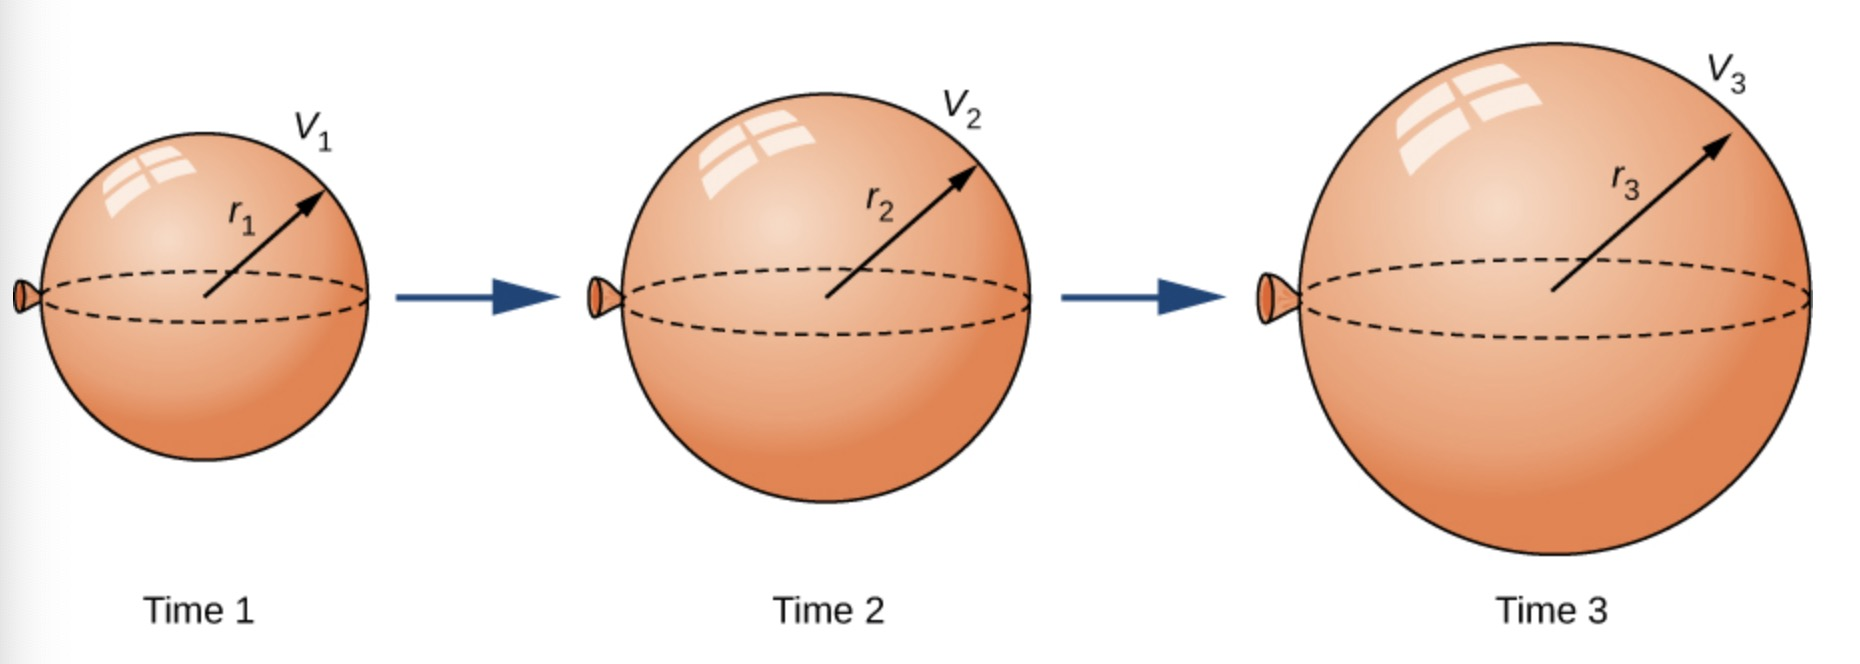
\includegraphics[width=0.90\linewidth]{Example_20.jpg} % Adjust the image width as necessary
    \captionof{figure}{}
    \label{fig:graph}
\end{minipage}

\newpage

\begin{tcolorbox}[colback=examplebg, colframe=red!75!black, title=\textbf{EXAMPLE 1: The Speed of an Airplane Tracked by Radar}, fonttitle=\bfseries, sharp corners]

An airplane is flying on a flight path that will take it directly over a radar tracking station. The distance \( s \) is decreasing at a rate of 400 miles per hour when \( s = 10 \) miles. What is the speed of the plane?

\begin{minipage}{\linewidth}
    \centering
    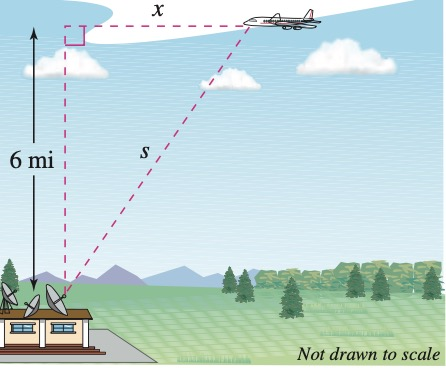
\includegraphics[width=0.28\linewidth]{Example_19.jpg} % Adjust the image width as necessary
    \captionof{figure}{}
    \label{fig:graph}
\end{minipage}

\tcblower
\textbf{Solution:}  
Let \( x \) be the horizontal distance from the station. Notice that when \( s = 10 \):
\[
x = \sqrt{10^2 - 6^2} = \sqrt{100 - 36} = 8 \, \text{miles}.
\]

\textbf{Given:}
\[
\frac{ds}{dt} = -400 \, \text{miles per hour when } s = 10.
\]

\textbf{Find:}
\[
\frac{dx}{dt} \, \text{when } s = 10 \text{ and } x = 8.
\]

\textbf{Equation:}
Using the Pythagorean Theorem:
\[
x^2 + 6^2 = s^2.
\]

Differentiate with respect to \( t \):
\[
2x \frac{dx}{dt} = 2s \frac{ds}{dt}.
\]

Solve for \( \frac{dx}{dt} \):
\[
\frac{dx}{dt} = \frac{s}{x} \frac{ds}{dt}.
\]

Substitute \( s = 10 \), \( x = 8 \), and \( \frac{ds}{dt} = -400 \):
\[
\frac{dx}{dt} = \frac{10}{8}(-400).
\]

Simplify:
\[
\frac{dx}{dt} = -500 \, \text{miles per hour}.
\]

\textbf{Conclusion:}
Since velocity is \( -500 \, \text{miles per hour} \), the \textbf{speed} of the plane is \( 500 \, \text{miles per hour} \).

\end{tcolorbox}



\begin{tcolorbox}[colback=examplebg, colframe=red!75!black, title=\textbf{EXAMPLE 2: Ripples in a Pond}, fonttitle=\bfseries, sharp corners]
A pebble is dropped into a calm pond, causing ripples in the form of concentric circles. The radius \( r \) of the outer ripple is increasing at a constant rate of 1 foot per second. When the radius is 4 feet, at what rate is the total area \( A \) of the disturbed water changing?

\begin{minipage}{\linewidth}
    \centering
    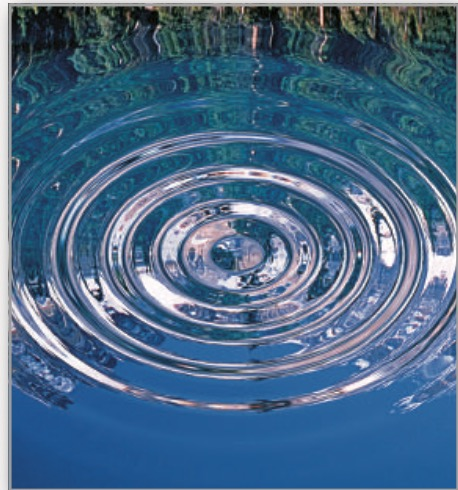
\includegraphics[width=0.30\linewidth]{Example_18.jpg} % Adjust the image width as necessary
    \captionof{figure}{}
    \label{fig:graph}
\end{minipage}

\tcblower
\textbf{Solution:}  
The variables \( r \) and \( A \) are related by:
\[
A = \pi r^2.
\]

\textbf{Given:}
\[
\frac{dr}{dt} = 1 \, \text{foot per second}.
\]

\textbf{Find:}
\[
\frac{dA}{dt} \, \text{when } r = 4.
\]

\textbf{Steps:}
Differentiate \( A = \pi r^2 \) with respect to \( t \):
\[
\frac{dA}{dt} = \frac{d}{dt}[\pi r^2].
\]

Using the chain rule:
\[
\frac{dA}{dt} = 2\pi r \frac{dr}{dt}.
\]

Substitute \( r = 4 \) and \( \frac{dr}{dt} = 1 \):
\[
\frac{dA}{dt} = 2\pi(4)(1).
\]

Simplify:
\[
\frac{dA}{dt} = 8\pi \, \text{square feet per second}.
\]

\textbf{Conclusion:}
When the radius is 4 feet, the area is changing at a rate of \( 8\pi \, \text{square feet per second} \).

\end{tcolorbox}


\newpage

\begin{tcolorbox}[colback=examplebg, colframe=red!75!black, title=\textbf{EXAMPLE 3: Rising Water Level in a Cone}, fonttitle=\bfseries, sharp corners]
A water tank has the shape of an inverted circular cone with a base radius of \( 2 \, \text{m} \) and height \( 4 \, \text{m} \). If water is being pumped into the tank at a rate of \( 2 \, \text{m}^3/\text{min} \), find the rate at which the water level is rising when the water is \( 3 \, \text{m} \) deep.




\tcblower
\textbf{Solution:} 

\textbf{Step 1: Relation Between Variables}
We are given:
\[
\frac{dV}{dt} = 2 \, \text{m}^3/\text{min}.
\]
We need to find \( \frac{dh}{dt} \) when \( h = 3 \, \text{m} \). The quantities \( V \) and \( h \) are related by the equation:
\[
V = \frac{1}{3} \pi r^2 h.
\]

Using similar triangles to eliminate \( r \):
\[
\frac{r}{h} = \frac{2}{4} \implies r = \frac{h}{2}.
\]

Substitute \( r = \frac{h}{2} \) into the volume equation:
\[
V = \frac{1}{3} \pi \left( \frac{h}{2} \right)^2 h = \frac{\pi}{12} h^3.
\]

\textbf{Step 2: Differentiate with Respect to \( t \)}
Differentiate \( V = \frac{\pi}{12} h^3 \) with respect to \( t \):
\[
\frac{dV}{dt} = \frac{\pi}{4} h^2 \frac{dh}{dt}.
\]

Solve for \( \frac{dh}{dt} \):
\[
\frac{dh}{dt} = \frac{\frac{dV}{dt}}{\frac{\pi}{4} h^2}.
\]

\textbf{Step 3: Substitute Known Values}
Substitute \( h = 3 \, \text{m} \) and \( \frac{dV}{dt} = 2 \, \text{m}^3/\text{min} \):
\[
\frac{dh}{dt} = \frac{2}{\frac{\pi}{4} (3)^2}.
\]

Simplify:
\[
\frac{dh}{dt} = \frac{2}{\frac{\pi}{4} \cdot 9} = \frac{8}{9\pi}.
\]

\textbf{Conclusion}
The water level is rising at a rate of:
\[
\frac{8}{9\pi} \approx 0.28 \, \text{m/min}.
\]
\end{tcolorbox}
\newpage






\subsection{Linear Approximation and Differentials}
\subsubsection{Tangent Line Approximations}

\textbf{}
Consider a function $f$ that is differentiable at $c$. The equation for the tangent line at the point $(c, f(c))$ is:

\[
y - f(c) = f'(c)(x - c)
\]

or, 

\[
y = f(c) + f'(c)(x - c)
\]

This is called the \textbf{tangent line approximation} of f at c

\begin{tcolorbox}[colback=examplebg, colframe=red!75!black, title=\textbf{EXAMPLE 1: Using a Tangent Line Approximation}, fonttitle=\bfseries, sharp corners]
\textbf{Find the tangent line approximation of \( f(x) = 1 + \sin x \) at the point \( (0, 1) \). Then use a table to compare the \(y\)-values of the linear function with those of \( f(x) \) on an open interval containing \( x = 0 \).}
\tcblower
\textbf{Solution:} The derivative of \( f \) is
\[
f'(x) = \cos x.
\]
First derivative

So, the equation of the tangent line to the graph of \( f \) at the point \( (0, 1) \) is
\[
y = f(0) + f'(0)(x - 0) = 1 + (1)(x - 0) = 1 + x.
\]
\end{tcolorbox}



\begin{tcolorbox}[colback=examplebg, colframe=red!75!black, title=\textbf{EXAMPLE 2: Using a Tangent Line Approximation}, fonttitle=\bfseries, sharp corners]
For a differentiable function \( g(x) \), it is known that \( g(2) = 7 \) and \( g'(2) = -3 \). Use the tangent line approximation at \( x = 2 \) to estimate \( g(2.1) \).
\tcblower
\textbf{Solution:} 
The equation of the tangent line at \( x = 2 \) is given by:
\[
L(x) = g(2) + g'(2)(x - 2).
\]

Substitute the known values:
\[
L(x) = 7 + (-3)(x - 2).
\]

To estimate \( g(2.1) \), substitute \( x = 2.1 \) into \( L(x) \):
\[
L(2.1) = 7 - 3(2.1 - 2)= 6.7.
\]


\end{tcolorbox}



\subsubsection{Underestimate or Overestimate}
\begin{table}[h!]
\centering
\renewcommand{\arraystretch}{1.5} % Adjust row spacing
\begin{tabular}{|c|c|c|}
\hline
\textbf{\( f'(x) = \text{Slopes of } f(x) \)} & \textbf{\( f''(x) \)} & \textbf{Tangent line to \( f \) gives an...} \\ \hline
Increasing & Positive & Underestimate \\ \hline
Decreasing & Negative & Overestimate \\ \hline
\end{tabular}
\caption{Relationship Between Derivatives and Tangent Line Behavior}
\end{table}


\begin{Note}{\textbf{A Common Mistake}}{}
\begin{itemize}
    \item We look to the \textbf{second derivative}, not the first derivative, to determine if a tangent line approximation is an overestimate or underestimate.
    \item A function \( f(x) \) could be increasing or decreasing, but we need to determine if the \textbf{slopes} of \( f(x) \) are increasing or decreasing to tell whether a tangent line will lie above or below the curve.
\end{itemize}
\end{Note}



\begin{tcolorbox}[colback=examplebg, colframe=red!75!black, title=\textbf{EXAMPLE 3: Tangent Line Approximation}, fonttitle=\bfseries, sharp corners]
For a differentiable function \( g(x) \), it is known that \( g(2) = 7 \), \( g'(2) = -3 \), and \( g''(2) = -5 \).

\begin{enumerate}
    \item[(a)] Use the tangent line approximation at \( x = 2 \) to estimate \( g(2.1) \).
    \item[(b)] Is the approximation in part (a) an overestimate or an underestimate of \( g(2.1) \)? 
\end{enumerate}
\tcblower
\textbf{Solution:} 
\textbf{Part (a): Tangent Line Approximation}
The equation of the tangent line at \( x = 2 \) is given by:
\[
L(x) = g(2) + g'(2)(x - 2).
\]

Substitute the known values:
\[
L(x) = 7 + (-3)(x - 2).
\]

To estimate \( g(2.1) \), substitute \( x = 2.1 \) into \( L(x) \):
\[
L(2.1) = 7 - 3(2.1 - 2)=6.7.
\]
\textbf{Estimated value of \( g(2.1) \): \( 6.7 \)}.

\textbf{Part (b): Overestimate or Underestimate?}
The second derivative \( g''(2) = -5 \) is \textbf{negative}, indicating that the slopes of \( g(x) \) are \textbf{decreasing}, meaning the approximation is an \textbf{overestimate}.




\end{tcolorbox}

\newpage
\subsubsection{Differentials}

\text{When the tangent line to the graph of \(f\) at the point \((c, f(c))\)}

\[
y = f(c) + f'(c)(x - c)
\]
is used as an approximation of the graph of \(f\), the quantity \(x - c\) is called the change in \(x\), and is denoted by \(\Delta x\). When \(\Delta x\) is small, the change in \(y\) (denoted by \(\Delta y\)) can be approximated as shown.

\[
\Delta y = f(c + \Delta x) - f(c) \approx f'(c)\Delta x
\]

\textit{Tangent line at \((c,f(c))\), Actual change in \(y\), Approximate change in \(y\)}

For such an approximation, the quantity \(\Delta x\) is traditionally denoted by \(dx\), and is called the \textbf{differential of \(x\)}. The expression \(f'(x)dx\) is denoted by \(dy\), and is called the \textbf{differential of \(y\)}.


\begin{Definition}{}{}
Let \( y = f(x) \) represent a function that is differentiable on an open interval containing \( x \). The \textbf{differential of \( x \)} (denoted by \( dx \)) is any nonzero real number. The \textbf{differential of \( y \)} (denoted by \( dy \)) is
\[
dy = f'(x) \, dx.
\]
\end{Definition}
\newpage

\subsection{L’Hospital’s Rule}
\begin{mytheorem}{L’Hospital’s Rule}{Squeeze Theorem}
Suppose \( f \) and \( g \) are differentiable and \( g'(x) \neq 0 \) on an open interval \( I \) that contains \( a \) (except possibly at \( a \)). Suppose that:
\[
\lim_{x \to a} f(x) = 0 \quad \text{and} \quad \lim_{x \to a} g(x) = 0
\]
or that:
\[
\lim_{x \to a} f(x) = \pm \infty \quad \text{and} \quad \lim_{x \to a} g(x) = \pm \infty.
\]

\textbf{(In other words, we have an indeterminate form of type \( \frac{0}{0} \) or \( \frac{\infty}{\infty} \).)}

Then:
\[
\lim_{x \to a} \frac{f(x)}{g(x)} = \lim_{x \to a} \frac{f'(x)}{g'(x)},
\]
if the limit on the right side exists (or is \( \infty \) or \( -\infty \)).

\end{mytheorem}


\begin{tcolorbox}[colback=examplebg, colframe=red!75!black, title=\textbf{EXAMPLE 1: Using L'hospital to find the Limit}, fonttitle=\bfseries, sharp corners]
Find:
\[
\lim_{x \to 1} \frac{\ln x}{x - 1}.
\]
\tcblower
\textbf{Solution:} 
Since:
\[
\lim_{x \to 1} \ln x = \ln 1 = 0 \quad \text{and} \quad \lim_{x \to 1} (x - 1) = 0,
\]
the limit is an indeterminate form of type \( \frac{0}{0} \), so we can apply L'Hospital's Rule:
\[
\lim_{x \to 1} \frac{\ln x}{x - 1} = \lim_{x \to 1} \frac{\frac{d}{dx}(\ln x)}{\frac{d}{dx}(x - 1)}.
\]

Differentiate the numerator and denominator:
\[
\lim_{x \to 1} \frac{\ln x}{x - 1} = \lim_{x \to 1} \frac{\frac{1}{x}}{1}.
\]

Simplify:
\[
\lim_{x \to 1} \frac{\ln x}{x - 1} = \lim_{x \to 1} \frac{1}{x} = 1.
\]
\end{tcolorbox}



\begin{tcolorbox}[colback=examplebg, colframe=red!75!black, title=\textbf{EXAMPLE 2: Using L'hospital to find the Limit}, fonttitle=\bfseries, sharp corners]
Calculate:
\[
\lim_{x \to \infty} \frac{e^x}{x^2}.
\]
\tcblower
\textbf{Solution:} 
We have:
\[
\lim_{x \to \infty} e^x = \infty \quad \text{and} \quad \lim_{x \to \infty} x^2 = \infty,
\]
so the limit is an indeterminate form of type \( \frac{\infty}{\infty} \). Using L'Hospital's Rule, we have:
\[
\lim_{x \to \infty} \frac{e^x}{x^2} = \lim_{x \to \infty} \frac{\frac{d}{dx}(e^x)}{\frac{d}{dx}(x^2)} = \lim_{x \to \infty} \frac{e^x}{2x}.
\]

Since \( e^x \to \infty \) and \( 2x \to \infty \) as \( x \to \infty \), the limit on the right side is also indeterminate. Applying L'Hospital's Rule again:
\[
\lim_{x \to \infty} \frac{e^x}{2x} = \lim_{x \to \infty} \frac{\frac{d}{dx}(e^x)}{\frac{d}{dx}(2x)} = \lim_{x \to \infty} \frac{e^x}{2}.
\]

Simplify:
\[
\lim_{x \to \infty} \frac{e^x}{2} = \infty.
\]
\end{tcolorbox}


\begin{tcolorbox}[colback=examplebg, colframe=red!75!black, title=\textbf{EXAMPLE 3: Using L'hospital to find the Limit}, fonttitle=\bfseries, sharp corners]

The table below gives selected values of a twice-differentiable function \( f(x) \):

\[
\begin{array}{|c|c|c|}
\hline
x & 5 & 3 \\ \hline
f(x) & 0 & -3 \\ \hline
f'(x) & 7 & 4 \\ \hline
\end{array}
\]

Find:
\[
\lim_{x \to 3} \frac{f(2x - 1)}{x^2 - 9}.
\]


\tcblower
\textbf{Solution:} 
First, substitute \( x = 3 \) into the numerator and denominator:
\[
f(2x - 1) \to f(2(3) - 1) = f(5) = 0, \quad x^2 - 9 \to 3^2 - 9 = 0.
\]

The limit is of indeterminate form \( \frac{0}{0} \), so we apply L'Hospital's Rule. Differentiate the numerator and denominator with respect to \( x \):
\[
\lim_{x \to 3} \frac{f(2x - 1)}{x^2 - 9} = \lim_{x \to 3} \frac{\frac{d}{dx}[f(2x - 1)]}{\frac{d}{dx}[x^2 - 9]}.
\]

Using the chain rule for the numerator:
\[
\frac{d}{dx}[f(2x - 1)] = f'(2x - 1) \cdot \frac{d}{dx}[2x - 1] = f'(2x - 1) \cdot 2.
\]

Differentiate the denominator:
\[
\frac{d}{dx}[x^2 - 9] = 2x.
\]

The limit becomes:
\[
\lim_{x \to 3} \frac{f'(2x - 1) \cdot 2}{2x}.
\]

Substitute \( x = 3 \):
\[
f'(2x - 1) \to f'(2(3) - 1) = f'(5) = 7.
\]

Substitute into the expression:
\[
\frac{f'(2x - 1) \cdot 2}{2x} \to \frac{7 \cdot 2}{2(3)} = \frac{14}{6} = \frac{7}{3}.
\]

\subsection*{Final Answer}
\[
\lim_{x \to 3} \frac{f(2x - 1)}{x^2 - 9} = \frac{7}{3}.
\]

\end{tcolorbox}
















\end{document}
